% !TEX TS-program = XeLaTeX
% use the following command:
% all document files must be coded in UTF-8
\documentclass[english]{textolivre}
% build HTML with: make4ht -e build.lua -c textolivre.cfg -x -u article "fn-in,svg,pic-align"

\journalname{Texto Livre}
\thevolume{15}
%\thenumber{1} % old template
\theyear{2022}
\receiveddate{\DTMdisplaydate{2022}{2}{28}{-1}} % YYYY MM DD
\accepteddate{\DTMdisplaydate{2022}{6}{2}{-1}}
\publisheddate{\DTMdisplaydate{2022}{8}{9}{-1}}
\corrauthor{Olga Fisenko}
\articledoi{10.35699/1983-3652.2022.38581}
%\articleid{NNNN} % if the article ID is not the last 5 numbers of its DOI, provide it using \articleid{} commmand 
% list of available sesscions in the journal: articles, dossier, reports, essays, reviews, interviews, editorial
\articlesessionname{articles}
\runningauthor{Fisenko et al.} 
%\editorname{Leonardo Araújo} % old template
\sectioneditorname{Daniervelin Pereira}
\layouteditorname{Leonado Araújo}

\title{Teaching Russian as a foreign language during the COVID-19 pandemic}
\othertitle{Ensino de russo como língua estrangeira durante a pandemia de COVID-19}
% if there is a third language title, add here:
%\othertitle{Artikelvorlage zur Einreichung beim Texto Livre Journal}

\author[1]{Olga Fisenko \orcid{0000-0002-3824-5535} \thanks{Email: \href{mailto:olfiss@list.ru}{olfiss@list.ru}}}
\author[2]{Zozulya Elena Alexandrovna \orcid{0000-0002-8601-8409} \thanks{Email: \href{mailto:zozulya.eag@bk.ru}{zozulya.eag@bk.ru}}}
\author[1]{Nikitina Vlada \orcid{0000-0003-0780-3140} \thanks{Email: \href{mailto:nikitina-vlada@internet.ru}{nikitina-vlada@internet.ru}}}
\author[3]{Bystrenina Irina Evgenevna \orcid{0000-0001-5424-691X} \thanks{Email: \href{mailto:iesh@rambler.ru}{iesh@rambler.ru}}}
\affil[1]{Peoples' Friendship University of Russia (RUDN University), Moscow, Russian Federation.}
\affil[2]{Plekhanov Russian University of Economics, Moscow, Russian Federation.}
\affil[3]{Russian State Agrarian University - Moscow Agricultural Academy, Moscow, Russian Federation.}

\addbibresource{article.bib}
% use biber instead of bibtex
% $ biber article

% used to create dummy text for the template file
\definecolor{dark-gray}{gray}{0.35} % color used to display dummy texts
\usepackage{lipsum}
\SetLipsumParListSurrounders{\colorlet{oldcolor}{.}\color{dark-gray}}{\color{oldcolor}}

% used here only to provide the XeLaTeX and BibTeX logos
\usepackage{hologo}

% if you use multirows in a table, include the multirow package
\usepackage{multirow}

% provides sidewaysfigure environment
\usepackage{rotating}

% CUSTOM EPIGRAPH - BEGIN 
%%% https://tex.stackexchange.com/questions/193178/specific-epigraph-style
\usepackage{epigraph}
\renewcommand\textflush{flushright}
\makeatletter
\newlength\epitextskip
\pretocmd{\@epitext}{\em}{}{}
\apptocmd{\@epitext}{\em}{}{}
\patchcmd{\epigraph}{\@epitext{#1}\\}{\@epitext{#1}\\[\epitextskip]}{}{}
\makeatother
\setlength\epigraphrule{0pt}
\setlength\epitextskip{0.5ex}
\setlength\epigraphwidth{.7\textwidth}
% CUSTOM EPIGRAPH - END

% LANGUAGE - BEGIN
% ARABIC
% for languages that use special fonts, you must provide the typeface that will be used
% \setotherlanguage{arabic}
% \newfontfamily\arabicfont[Script=Arabic]{Amiri}
% \newfontfamily\arabicfontsf[Script=Arabic]{Amiri}
% \newfontfamily\arabicfonttt[Script=Arabic]{Amiri}
%
% in the article, to add arabic text use: \textlang{arabic}{ ... }
%
% RUSSIAN
% for russian text we also need to define fonts with support for Cyrillic script
% \usepackage{fontspec}
% \setotherlanguage{russian}
% \newfontfamily\cyrillicfont{Times New Roman}
% \newfontfamily\cyrillicfontsf{Times New Roman}[Script=Cyrillic]
% \newfontfamily\cyrillicfonttt{Times New Roman}[Script=Cyrillic]
%
% in the text use \begin{russian} ... \end{russian}
% LANGUAGE - END

% EMOJIS - BEGIN
% to use emoticons in your manuscript
% https://stackoverflow.com/questions/190145/how-to-insert-emoticons-in-latex/57076064
% using font Symbola, which has full support
% the font may be downloaded at:
% https://dn-works.com/ufas/
% add to preamble:
% \newfontfamily\Symbola{Symbola}
% in the text use:
% {\Symbola }
% EMOJIS - END

% LABEL REFERENCE TO DESCRIPTIVE LIST - BEGIN
% reference itens in a descriptive list using their labels instead of numbers
% insert the code below in the preambule:
%\makeatletter
%\let\orgdescriptionlabel\descriptionlabel
%\renewcommand*{\descriptionlabel}[1]{%
%  \let\orglabel\label
%  \let\label\@gobble
%  \phantomsection
%  \edef\@currentlabel{#1\unskip}%
%  \let\label\orglabel
%  \orgdescriptionlabel{#1}%
%}
%\makeatother
%
% in your document, use as illustraded here:
%\begin{description}
%  \item[first\label{itm1}] this is only an example;
%  % ...  add more items
%\end{description}
% LABEL REFERENCE TO DESCRIPTIVE LIST - END


% add line numbers for submission
%\usepackage{lineno}
%\linenumbers

\begin{document}
\maketitle

\begin{polyabstract}
\begin{abstract}
Foreigners coming to the Russian Federation must learn Russian as a foreign language to be able to enter professional programs at Russian higher education institutions. Unfortunately, many foreign students entering medical faculties often lack the required academic level of proficiency in Russian. For this purpose, Russian higher education institutions develop online courses and introduce additional digital resources into the educational process. The need for high-quality educational content has escalated by the COVID-19 pandemic. That is why the Peoples’ Friendship University of Russia invites foreign students in biomedical pre-university programs to take an online course in the scientific style of the Russian language from the elementary level to B1. The objective of this study was twofold: first, we attempted to examine how the students’ attitude towards Russian as a foreign language, motivational sphere, and performance change as they take the course; next, we examined the level of satisfaction of foreigners with such courses in two years - in 2018, during the pre-pandemic period, and in 2021, when the COVID-19 pandemic had a clear impact on the extensive use of distance learning. For this purpose, we used modified questionnaires by \textcite{orlov_kolmogorov_2014}, and created a questionnaire all foreign students were asked to answer upon completing the courses. The study showed that foreign students of the biomedical profile who study at preparatory faculties on the proposed courses in 2018 and 2021 exhibited significant differences in the motivational sphere, the nature of their attitude towards the applied online courses. These findings allow us to conclude that the applied online courses are a valid supplemental form of training that can be used during any situation that causes in-person instruction to be impractical and can be used as material for independent work within the traditional classroom teaching system.

\keywords{Language of the major \sep Online learning \sep Covid-19 pandemic \sep Foreign learners \sep Russian as a second language}
\end{abstract}

\begin{portuguese}
\begin{abstract}
Os estrangeiros que chegam à Federação Russa devem aprender russo como língua estrangeira para poder ingressar em programas profissionais em instituições de ensino superior russas. Infelizmente, muitos estudantes estrangeiros que ingressam em faculdades de Medicina geralmente não possuem o nível acadêmico necessário de proficiência em russo. Por isso, as instituições de ensino superior russas desenvolvem cursos \textit{on-line} e introduzem recursos digitais adicionais no processo educacional. A necessidade de conteúdo educacional de alta qualidade aumentou devido à pandemia do COVID-19. É por isso que a Peoples’ Friendship University da Rússia convida estudantes estrangeiros em programas pré-universitários biomédicos para fazer um curso \textit{on-line} no estilo científico da língua russa do nível elementar ao B1. O objetivo deste estudo é duplo: primeiro, tentamos examinar como a atitude dos alunos em relação ao russo como língua estrangeira, a esfera motivacional e o desempenho mudam à medida que fazem o curso; em seguida, examinamos o nível de satisfação dos estrangeiros com esses cursos em dois anos - em 2018, no período pré-pandemia, e, em 2021, quando a pandemia de COVID-19 teve um impacto claro no uso extensivo do ensino a distância. Para tanto, utilizamos questionários modificados de \textcite{orlov_kolmogorov_2014}, e criamos um questionário que todos os alunos estrangeiros deveriam responder ao concluir os cursos. O estudo mostrou que estudantes estrangeiros do perfil biomédico que cursam faculdades preparatórias nos cursos propostos em 2018 e 2021 apresentaram diferenças significativas na esfera motivacional, na natureza de sua atitude em relação aos cursos \textit{on-line} aplicados. Esses achados permitem concluir que esses cursos são uma forma complementar válida de treinamento que pode ser usada em qualquer situação que torne o ensino presencial impraticável e pode ser usado como material para trabalho independente dentro do sistema tradicional de ensino presencial.

\keywords{Língua da graduação \sep Aprendizado \textit{on-line} \sep Pandemia de COVID-19 \sep Alunos estrangeiros \sep Russo como segunda língua}
\end{abstract}
\end{portuguese}
% if there is another abstract, insert it here using the same scheme
\end{polyabstract}

\section{Introduction}\label{sec-intro}
The COVID-19 pandemic which began in the winter of 2020 has necessitated the search for new online educational technologies that would expand the opportunities for mastering the language of the major using open access via the Internet. Professors of both public and private higher educational institutions are interested in high-quality teaching using online technologies, especially when full-time education forms cannot be the only option for organizing training sessions, as is currently the case in many higher educational institutions throughout the world. Online learning environments (OLE) including learning management systems (LMS) and massive open online courses (MOOCs) are gaining traction \cite{barcena_role_2015,uddin_systematic_2021}. The new reality in which higher education institutions have to organize the education process creates conditions for testing the created Massive Open Online Courses (MOOCs) for their educational effectiveness, building up academic motivation in students on a wider scale than usual. Therefore, the purpose of this study is to evaluate how a high-quality educational online resource as a means of learning a language for a future profession contributes to satisfying the students’ cognitive needs, creates a persistent motivation to learn the language of their major, and affects the students’ academic performance.

\textcite{luik_are_2021} in their study argue that the motivation of students enrolling in MOOCs is an essential factor that correlates with student dropout rates. The most important condition for increasing students’ motivation as they use MOOCs is finding the most effective ways to use their benefits.
 
It is widely believed by scientists that the students’ motivational sphere plays an important role in the process of learning a foreign language. Studying the relationship between learning, motivation and self-control allows us to understand the reasons why some foreign languages are easier to learn than others \cite{zhu_relationship_2022}. Specially developed program of the virtual learning environment in the context of the Emergency Remote Teaching (ERT) strategy implementation imply the development of a contingency plan \cite{rodes_teacher_2021}. Difficulties arise in establishing feedback that requires individual support of the students. Various education approaches existing in the higher professional education system contribute to an increase in the quality of language massive open online courses.

Massive open online courses have a low student-to-staff-ratio, so the students must be capable of learning independently.

\textcite{rodes_teacher_2021} examined the relationship between motivation, self-control, and the use of MOOC learning strategies by learners.

Volunteers were surveyed after completing three MOOCs. A survey of 470 participants showed that motivation has a positive effect on self-control, self-management, and learning strategies.
The findings highlight the urgent need to improve self-control skills to further develop self‑management skills in MOOCs.
Experimental materials on the implementation of Linguistics MOOCs (LMOOCs) in the education process provided herein were obtained for the pre-pandemic year 2018 and the year 2021, when the COVD-19 pandemic spread around the world. In the 2017–2018 academic year, LMOOCs (Language MOOCs) were supplementary to the main course. The curriculum did not allocate time for it whereas in the 2020–2021 academic year, about 40 \% of the study time was allocated for LMOOC training. It means that MOOCs began to be seen as part of online education, of the traditional classroom education system, and distance learning programs.

\textbf{Study hypothesis}: Teaching the academic style of the Russian language amid the fight against the pandemic will be more efficient if up to 40 \% of the time, according to our hypothesis, is allocated for unsupervised work using the LMOOC “Russian Language for a Future Specialist, Biomedical Profile”. Successful completion of the LMOOC (the degree of proficiency in Russian as a foreign language, academic performance) depends on the students’ motivational sphere and attitude to the LMOOC educational environment. The LMOOC efficiency indicators included the level of proficiency in the language of the major, interest in the studied course, achievement motivation and degree of satisfaction with the course.

The study was conducted in order to measure the relationship between achievement motivation, proficiency in the language of the major, academic performance, and the degree of satisfaction with the LMOOC in foreign students learning Russian as the language of the major. The study is based on comparing polling data and surveys of foreign students studying at the Peoples’ Friendship University of Russia in years 2017–2018 and 2020–2021.

\section{Theoretical framework of the study}\label{sec-normas}

This section contains an analytical review of the scientific literature on the specific aspects of the MOOC concepts.

\subsection{General characteristics of MOOCs}

Massive open online courses (MOOCs) are gaining practical importance during the pandemic. The advantages of MOOCs include a wider audience coverage, as well as resolving the problem of access to higher education. It expands the boundaries of education making it more accessible to people living in one country and wishing to study in another one. The main objective of MOOCs is to attract the maximum number of students. The motives that make students choose a particular MOOC may be determined by their personal demand, their desire for intellectual development, and the possibility of career advancement \cite{hew_students_2014}.

MOOCs retain features of an academic course such as curriculum, learning objectives, course materials, activities, teacher-student interaction, student-student interaction, etc. \cite[p. 107]{martin-monje_researching_2021}.

While the objectives of online and classroom education are the same, the teaching methods are very different. Online learning does not require classrooms, campuses, libraries, numerous teachers and service personnel. However, it requires a powerful computer network to be able to solve complex problems and adapt to the students’ needs \cite{kadlecik_efficacy_2020}. The conducted studies on digital learning have demonstrated their potential. Today, MOOCs are viewed as a major education trend. MOOCs are often used as a component of blended learning.

However, the MOOC organizers face the problem of loss of students. The evaluation of the results of taking MOOCs showed that there were students who failed to complete each course. Researchers have proven that many students enrolling in MOOC courses show a decrease in interest in learning at the end of the first month of learning and during weeks 10 to 11 of the course \cite{a_shukor_using_2019}. MOOCs also have significant drawbacks related to students lacking access to high-quality Internet resources in some regions, poor involvement of weaker students, etc. Thus, the main problems associated with the implementation of MOOCs include: high dropout rates, insufficient motivation, low quality of knowledge, etc. \cite{feklistova_learners_2021} conducted a study to determine which factors affect the dropout rate and to examine the factors that affect the involvement of students in the course as well as overcoming challenges arising during the learning process. Successful completion of a MOOC is influenced by many internal and external factors. The former ones include the problem of self-management: managing time, resources, and support \cite{zhu_enhancing_2021}. The latter ones include the problems of the educational product quality, and satisfaction with its content. An analysis by \textcite[p. 3459-3461]{albelbisi_self-regulated_2021} using partial least squares structural equation modeling (PLS-SEM) showed that the system quality has a positive effect on satisfaction, satisfaction and service quality have a positive effect on self-controlled learning and, finally, the quality of the system has an indirect impact on the SRL through satisfaction.

\textcite{fan_research_2021} describes the advantages of MOOCs. Firstly, it is a more flexible, deadline-free format of training where students choose the training content and schedule themselves. Secondly, MOOCs are created by well-known professors who meticulously plan the MOOC content. Thirdly, they are interactive, vivid, graphic, and have unconventional material presentation. MOOCs are represented by short and very concise videos that do not take up much time to watch. Having analyzed the existing MOOCs, \textcite[p. 1-2]{estebas-vilaplana_role_2020} determined the following criteria: 1) formal (credit bearing and tightly curriculated) MOOCs, 2) semi-formal (not part of a degree but may grant credits) and 3) non-formal MOOCs (with no credits and no curriculum alignment).

Types, target participants, content and resources involved are considered as the differentiating principles of MOOCs. \textcite{pilli_taxonomy_2016} consider the massiveness and openness of MOOCs to be the main criteria as follows: 1) small scale and less open; 2) small scale and more open; 3) large scale and less open; 4) large scale and more open. The main types of MOOCs are MOOCs conducted by colleges and MOOCs conducted by higher education institutions \cite{berestova_mooc_2021}.

Because digital technologies are well developed, we can consider MOOCs as a form of education. On the one hand, MOOCs allow one to organize distance learning and control the level of mastering the material, and on the other hand, the lack of a methodological framework in MOOCs makes it difficult to create courses meeting the needs of students, having a methodological framework, and increasing the motivation to learn the subject.

\subsection{Language MOOCs}\label{sec-conduta}
The development of open educational resources has increased the number of foreign language learning courses. An LMOOC is a special educational environment where the degree of student involvement in the educational process is crucial.
\textcite[p. 27–28]{sokolik_2_2014} describes the following criteria of a successful LMOOC:

\begin{enumerate}
    \item Maximization of engagement and interaction;
    \item Facilitation of self-organized learning;
    \item Creation of an instructor presence;
    \item Use of videos for engagement;
    \item Definition of success;
    \item Matching of the course goal and its assessment.
\end{enumerate}
 
It is the language online courses that are currently considered the most adequate way to access high-quality education during the pandemic. Today, LMOOCs are specialized online courses for learning a second language.

Language courses are designed to cover more languages. During the COVID-19 pandemic, foreign languages were included in the 10 most popular courses by demand. The most popular languages are Chinese, English, Spanish, Italian, and Portuguese. Many courses are designed for a certain level of language proficiency, such as A1, A2, B1, etc. \cite{shah_second_2020}.

Currently, many higher education institutions use LMOOC to attract foreign undergraduate and graduate students. About a half of all the MOOCs are focused on foreign languages. Many courses quickly gained popularity and are highly rated by students. However, many problems remain unresolved. They include the challenges related to making them a profitable education business.

A distinctive feature of the offered LMOOCs is their modular organization making it possible to systematize educational materials.

\textcite{jitpaisarnwattana_learners_2021} argue that all LMOOCs can be divided into two main types: xMOOC and cMOOC. While the first type implies short videos with closed tasks and comprehension tests, the second one is more flexible and creates opportunities for customized learning based on interaction between students and teacher-student interaction. However, practice shows that students fail to capitalize on these opportunities.

\textcite{xiao_motivation_2021} focuses on the MOOC platform and the Internet university of the future Xuetangx.com. The existing MOOCs are integrated into practical training, providing training in professional skills.

\textcite{estebas-vilaplana_role_2020} cite a LMOOC called “The Acquisition of English Pronunciation through Songs and Literary Texts” used as supplementary material for teaching English to Spanish-speaking students as an example of LMOOC use. The LMOOC is a hands-on experience of teaching English phonetics and studying the implications of combining formal tuition with implicit learning. The peculiarity of this LMOOC is its semi-formal nature. It contains supplementary materials for the English Pronunciation course as part of the Degree in English Studies held at the Universidad Nacional de Educación a Distancia (UNED) in Spain.

Mobile Open Social Learning for Languages (MOSL4L) is a space for learning a foreign language combining three elements: mobile, open, and social. It offers changes to language programs taking into account the current communication problems \cite{kukulska-hulme_mobile_2021}.

Studies by \textcite{pareja-lora_learning_2016,vorobyeva_language_2018} showed that LMOOC appeared effective in teaching reading and listening skills. It is much more difficult to develop writing and speaking skills as they require feedback and oral practice.


\subsection{The role of motivation in developing persistent interest in LMOOC}\label{sec-fmt-manuscrito}
There are three groups of motivation: 1) needs and instincts (primary sources of activity); 2) motives as such (reasons for choosing a specific behavior); 3) feelings and attitudes (regulators of activity dynamics) \cite{petrovskiy_brief_1985,solso_experimental_2003}. In Russian science, motivation is studied based on a subject-object scheme within the activity approach. According to Rubinstein, behavior motives are associated with the mental reflection of a need and are based not on individual needs, but on social ideology, ideas about the right and the lawful \cite[p. 444]{rubinstein_fundamentals_2000}. In Leontyev’s concept, a motive cannot exist outside an activity. A motive determines the meaning of any activity. On the one hand, motives drive and guide activity; on the other hand, they give meaning to the activity. A motive means “an entity in which need is concretized under the given conditions and at which the activity is aimed as an incentive” \cite[p. 290]{leontyev_activity._1975}. Bozovic’s understanding of a motive as an object of the outside world, an idea, an experience distinguishes groups of social motives within motivation. It also associates the development of motivation for human behavior with the transformation of physical needs into spiritual ones \cite{bozhovich_personality_1968}. According to \textcite{manukyan_individual_1984}, a motive as an activity vector with a specific objective content is concretized in relation to the activity goal. Further development of the motivation theory is found in the work of Dodonov. A need means an individual’s internal life activity program. A motive is the result of the process of correlating the individual life activity program with social values \cite{dodonov_structure_1984}.

Such studies as the \posscite{deci_facilitating_2008} show that the internal motivation which correlates with the personal responsibility of the education process subjects allows the latter to control the learning process. The self-identification of the students is crucial. Students reconsider the activity goals and objectives in the process of self-identification. A hierarchy is built within the activity structure. The activities aimed at preparation for adulthood comes first. Life planning is based on self‑regulation and self-control abilities \cite{leontyev_psychology_2000}. Self-control and self-management are also part of the responsibility for building a personal learning strategy.

Self-controlled learning is a process where learners initiate their own cognitive activities in order to achieve their learning objectives \cite{zimmerman_social_1989}. The online education environment requires an especially high level of self-regulation.

\textcite{winne_self-regulating_2003} view deficiencies in learning strategies as disadvantages of the MOOC education environment. \textcite{lust_regulation_2013} demonstrated that only 3 \% of learners used MOOC resources effectively. Moreover, only 7 \% to 10 \% of learners complete MOOCs \cite{daniel_making_2012}, which also indicates a lack of their motivation for self-study using MOOCs. Having examined the role of motivation, anxiety, and beliefs in self-efficacy in learning Spanish using LMOOCs, \textcite{barkanyi_motivation_2021} concluded that internally motivated students are more likely to complete the course than those who started learning the language to advance their career or further their education. However, no direct correlation was found between motivation and other studied variables.

Lack of communication with peers or teachers has an adverse effect on the motivation to learn a language and results in high dropout rates \cite{khalil_moocs_2014}.

The level of motivation to learn using LMOOCs is influenced by the background experience of the students, their individual psychological make-up, and the degree of personal and social significance of the education process. The teacher also plays an essential role in the process of motivating. A high level of motivation is crucial for activating self-regulation skills. Motivation influences the performance of MOOC students.

\textcite{yen_framework_2018} associates the skills of building a self-controlled system with the time management skills. There are 8 components: 1) learning plans (students should have clear learning objectives); 2) recording and sharing about learning progress (it is important to remember that the learning motivation is influenced by the student’s awareness of the educational progress during learning); 3) assessment (crucial elements of the motivational sphere are reflection, perception of the education results); 4) human feedback (feedback is a necessary education component); 5) machine feedback; 6) visualization (a self-controlled system means availability of and adherence to a learning concept); 7) scaffolding/prompts; and 8) agents.

\section{Teaching Russian as Second Language}\label{sec-formato}
Teaching foreigners the scientific style of the Russian language is a challenging task due to its complex formalized structure, the wide use of complex linguistic structures that are not inherent in the spoken language, and special terminology. Developing methods and techniques for teaching the language for scientific and professional purposes began in Russia more than 60 years ago. It was then that the need to create a subject-oriented Russian language was first voiced. Teaching the scientific style of speech to foreigners involves the study of major subjects in Russian. Teaching the language for scientific and professional purposes to foreigners is a crucial part of the general education process at the stage of pre-university preparation of foreign students for enrollment and studying in higher education institutions of the Russian Federation.

It is particularly challenging for foreign students training to be healthcare professionals, biologists, agronomists, etc., to learn Russian as the language of the major. The system of training foreign students of the biomedical profile implies teaching the Russian language at a level that would allow them to study major subjects in the language of the country where they intend to receive higher education and developing skills needed to obtain medical knowledge within the framework of higher education in the future.

Russian as a foreign language in the system of pre-university training of biomedical students is integrated with Biology, Mathematics, Physics, Chemistry, and changes from a purely linguistic phenomenon to an interdisciplinary one. Teaching the language of the major is even more complicated amidst the rise of online technologies making it difficult to establish immediate feedback with the students. The pandemic years have shown that, despite the existing LANGUAGE TEACHING programs for scientific and professional purposes to foreign students of preparatory faculties, these students still lack sufficient language training in the scientific sphere. Many Russian language teachers point out the insufficient level of knowledge of the necessary terms, language structures that would allow foreigners to master new language material based on the studied models and to engage in educational communication in the language of their future profession. Professors of special disciplines teaching first-year students of main faculties also express their dissatisfaction with the quality of training of foreign students in the field of scientific speech style.

The foregoing indicates the need to develop new advanced pedagogical technologies that would contribute to a higher degree of proficiency in the language of the major already at the pre-university stage. One possible way to teach the scientific style of the language of the major to foreigners is the development of LMOOCs which can either form a mandatory component of the educational process and be included in the credit system or supplement the existing classroom or online courses.


\section{Methods}\label{sec-modelo}
The objective of the study is to identify the motives that influence the learning behavior motivation. Questionnaires and polls were used as the sources of empirical data. The survey was conducted twice: at the beginning and upon completion of the training. At the first stage, we received data on the initial intentions, motivational and semantic constructs of the achievement motivation of foreign students studying at preparatory faculties. Widely used questionnaires were used as the basis, which confirms the validity of the tests. The test results were analyzed only when the experiment participants confirmed their understanding of the questions. This evidenced the reliability of the tests.

\begin{enumerate}
    \item Orlov – Sosnovsky’s questionnaire aimed at studying the social motivational and semantic constructs of foreigners. The questionnaire contained 98 statements with which foreigners enrolling in MOOCs were asked to agree or disagree. The highest score corresponds to the highest intensity of the need for achievements.
    \item Modified Ilyina’s “Questionnaire for Studying the Higher Education Motivation”. There are three scales: “knowledge acquisition” (desire to acquire knowledge, curiosity); “mastering the language of the major” (the desire to master the language of the major as a means to obtain professional knowledge and develop important professional competencies); “enrollment in a specialized higher education institution for the chosen profession” (the desire to be admitted to a higher education institution, receive a diploma and formal education, and search for workarounds for passing exams and getting credits).

The obtained statistical data reflecting the strength of educational activity motives were subjected to a factor analysis. Factors have been weighed and described. Analytical and factorial motivation structures have been compared.

The nature of learning activity motivation was determined in two groups of students. The conclusion about the motivation level and nature was made based on the comparison of scores on the “knowledge acquisition”, “mastering the language of the major” scales. If the total scores on the “knowledge acquisition”, “mastering the language of the major” scales exceed the “enrollment in a specialized higher education institution for the chosen profession” scale, it was concluded that the foreigners’ education motivation was adequate. Foreigners of the two groups were asked to complete the questionnaires twice: at the beginning and upon completion of the LMOOC “Russian Language for a Future Specialist. Biomedical Profile”.

\item Final performance in the LMOOC “Russian Language for a Future Specialist. Biomedical Profile”. All the participants took the final test, regardless of how far they advanced in the LMOOC “Russian Language for a Future Specialist. Biomedical Profile”.

\item A survey on the degree of satisfaction with the LMOOC “Russian Language for a Future Specialist Biomedical Profile” with open-ended questions.
\end{enumerate}

The experiment design was in accordance with the regulatory standards of the country where the experiment was conducted.

\subsection{General characteristics of the respondents}\label{sec-organizacao}
A total of 160 people took part in the experiments ($n = 160$). The number of experiment participants in each group was limited to 80 people ($n₁ = 80$ and $n₂ = 80$). Excessive questionnaires were excluded from the count. The first group consisted of foreign students of the biomedical profile who studied at a preparatory faculty in the 2017–2018 academic year ($n = 80$). The average age of the respondents was 22.7 years.

The second group consisted of foreign students of the biomedical profile who studied at a preparatory faculty in the 2020–2021 academic year ($n = 80$). The average age of the respondents was 21.3 years. It should be noted that the groups were the same in terms of composition and similar in terms of age, making the experiment more reliable.

The first group of foreigners studied in Russian higher education institutions full-time. Online technologies were considered as supplementary materials to the classroom education system and were optional. The second group of foreigners studied in Russian higher education institutions online, so the LMOOC “Russian Language for a Future Specialist. Biomedical Profile” was a mandatory part of the language training system for foreign students.

\subsection{General description of the LMOOC “Russian Language for a future specialist biomedical profile”}\label{sec-organizacao-latex}
“Russian Language for a Future Specialist. Biomedical Profile” is a LMOOC intended for self‑directed learning of the scientific style of speech by foreign students of preparatory faculties under mixed/hybrid/combined education conditions. The course duration is 16 hours.

The LMOOC “Russian Language for a Future Specialist. Biomedical Profile” is designed to teach a language for special purposes (LSP) which, pursuant to \textcite{chapelle_genre_2018}, is understood as special language training focused on characteristic linguistic properties, discursive practices, and communication skills used by certain groups.

At the first stage of the experiment in the 2017–2018 academic year, LMOOC was offered as auxiliary material.

At the second stage of the experiment in the 2020–2021 academic year, it was proposed to transfer 40 \% of the academic process from classrooms of the preparatory department to the virtual space of the LMOOC “Russian Language for a Future Specialist. Biomedical Profile”. At the same time, on-site lessons were not excluded completely. The education process implied alternation of direct and hybrid training of foreign students.

The LMOOC “Russian Language for a Future Specialist. Biomedical Profile” is designed for foreign students at pre-university programs. The main target population includes students enrolled in biomedical programs.

The main criterion for the development of the LMOOC “Russian Language for a Future Specialist. Biomedical Profile” is the customization of education, which means considering the personal potential of the students and their individual language learning needs, which makes mastering the educational program individually significant. The LMOOC is structured considering the personal educational needs associated with learning new vocabulary, the basic structures of the language of the future profession. Learning the scientific style of speech allows foreigners to self-regulate the language learning process. They regulate the volume of the studied material themselves.

The next most important criterion for structuring the LMOOC is building a customized education environment offering conditions needed to satisfy the personal needs of foreign students. Customized learning is focused on recognition of education as a value. The scientific speech style course contributes to the self-identification of the students within the chosen profession. Customization of the LMOOC “Russian Language for a Future Specialist. Biomedical Profile” creates conditions needed for training of each student considering their individual capabilities, education motives, interests. All this contributes to the development of a certain degree of tailoring to the needs of the individual student in the LMOOC education process. Customization is related to individuality and autonomy of the students and is aimed at developing their skills to self‑direct their educational behavior patterns. Personal mechanisms are formed based on self‑regulation processes. The course is designed to develop the potential of each consumer of education services.

The LMOOC is also tailored to the needs of the Language of the Major curriculum and the educational needs of each student. The course is clearly structured - it has a step-by-step assessment of the degree of mastering the training material. Topical units consist of several lessons under a pre-developed program.

Each unit contains video and audio materials: logically complete small parts easily comprehensible for foreign listeners, targeting visual, auditory, and emotional memory. Small audio-visual fragments of lessons make it easier to understand and memorize the new material. Fragment‑by‑fragment presentation of the multimedia content contributes to the development of word recognition skills and the ability to use them in speech.

Online lessons and topical units include text assignments. By completing them correctly, foreign students obtain access to a new unit of educational information. If they make mistakes when taking intermediate tests, they can refer to grammatical and reference materials, video lessons and audio materials. The LMOOC “Russian Language for a Future Specialist. Biomedical Profile” contains three types of tests: subject-oriented, grammar-oriented, and combined ones.

In this study, we wanted to see whether the LMOOC can support motivation to learn the language of the major. The course consists of 4 units: “Mathematics”, “Chemistry”, “Physics”, and “Biology”. All the units included learning audio materials. Each unit introduced the students to new vocabulary. Particular attention is paid to the development of pronunciation skills. Grammar is introduced based on the educational needs. LMOOC participants can listen to and watch the materials as many times as needed. After each lesson and unit, there are control tests aimed mostly at the self-control of the degree of understanding of each lesson of the course. The LMOOC ends with a final test we can use to judge the successful completion of the course. Foreigners continue to study the declension system and prepositions of the Russian language. Particular attention is paid to the singular and plural forms of the Genitive and Dative cases. They develop pronunciation and writing skills. Particular attention is paid to the development of communication skills in the education sphere. If necessary, foreigners can refer to online dictionaries, the links to free versions of which are available in the course.

After completing the LMOOC course, the participants were asked to express their opinion on the course structure, their expectations regarding the learning outcomes, its importance in mastering the language of the major. Throughout the course, participants could ask the scientific language teachers organizing the educational process for help.

\section{Results}\label{sec-titulo}
\subsection{Sample normality testing}
Based on the studies by \textcite{orlov_kolmogorov_2014}, non-parametric Kolmogorov–Smirnov tests were used to measure the normality of the studied samples. Our sample size was 80 people per group, which corresponded to the necessary condition of n$_{1,2}$ $\ge 50$. We compared the obtained data with the standard normal distribution.

\begin{table}[htbp]
\begin{threeparttable}
\caption{Kolmogorov–Smirnov Normality Test.}
\label{tab01}
\centering
\begin{tabular}{l c c}
\headrow \thead{Groups} & \thead{statistics} & \thead{asymptotic value} \\
achievement motivation in group 1 after completing the LMOOC     & 1.051 & 0.221   \\
achievement motivation in group 2 after completing the LMOOC     & 1.298  & 0.69  \\
\end{tabular}
\source{Own elaboration}
\end{threeparttable}
\end{table}

As is shown in \Cref{tab01}, if the asymptotic value is greater than 0.05 ($p > 0.05$), the distribution is considered normal.

\subsection{Evaluation of social motivational and semantic constructs}
The motivational sphere was examined based on a qualitative and quantitative analysis of the data obtained using the Yu. M. Orlov–B. A. Sosnovsky questionnaire.

The intensity of needs for achieving security, knowledge, affiliation, etc. of foreigners studying in the 2017–2018 academic year are shown in \Cref{fig01}.

\begin{figure}[htbp]
 \centering
 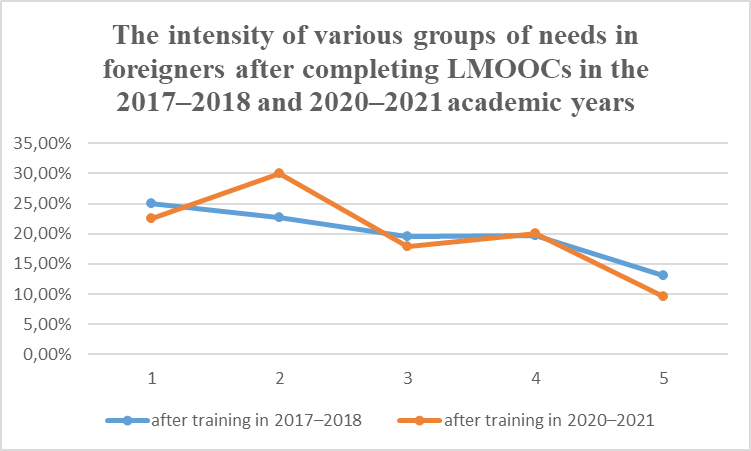
\includegraphics[width=0.85\textwidth]{Fig1.png}
 \caption{Intensity of groups of needs in foreigners after completing LMOOCs.}
 \label{fig01}
 \source{Own elaboration.}
\end{figure}

Needs were divided in five groups: 1) material needs; 2) need for self-actualization; 3) need for belonging and love; 4) need for security; 5) need for self-respect.

A comparative analysis of the intensity of needs in foreigners who studied in 2017–2018 showed minor changes in the intensity before and after training, which suggests that the LMOOC “Russian Language for a Future Specialist. Biomedical Profile” did not have a significant impact on the motivational sphere of the students.

The intensity of needs of foreigners studying in the 2020–2021 academic year are shown in \Cref{fig02}.

\begin{figure}[htbp]
 \centering
 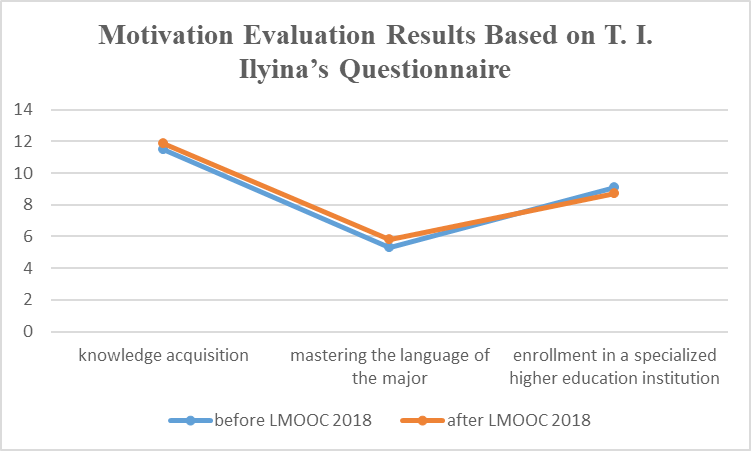
\includegraphics[width=0.85\textwidth]{Fig2.png}
 \caption{Motivation evaluation results.}
 \label{fig02}
 \source{Own elaboration.}
\end{figure}

1) material needs; 2) need for self-actualization; 3) need for belonging and love; 4) need for security; 5) need for self-respect.

The 2020–2021 study group showed an increase in the importance of the need for self‑actualization. Self-actualization is defined as young people’s personal growth, the desire to fulfill their professional potential. The material needs associated with further benefits of receiving education are rather significant. The need for security is also important in the 2020–2021 study group. This is the need for stability, organization, law and order, predictability of events, and freedom from threatening factors such as fear, illness, etc.

A comparative analysis of the intensity of different groups of needs in 2018 and 2021 showed significant differences in the degree of their intensity (\Cref{fig03}).

\begin{figure}[htbp]
 \centering
 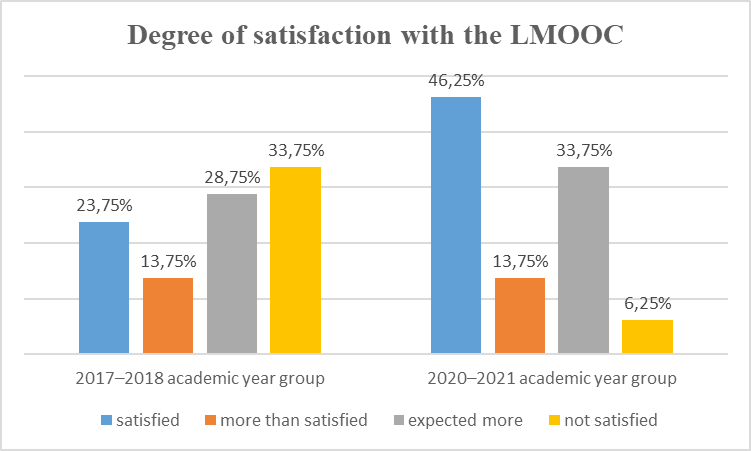
\includegraphics[width=0.85\textwidth]{Fig3.png}
 \caption{Degree of satisfaction with the LMOOC.}
 \label{fig03}
 \source{Own elaboration.}
\end{figure}

1) material needs; 2) need for self-actualization; 3) need for belonging and love; 4) need for security; 5) need for self-respect.

After completing the LMOOC “Russian Language for a Future Specialist. Biomedical Profile”, foreigners of the 2020–2021 study group showed higher needs for self-actualization and professional growth compared to the 2017–2018 study group. Both the individual psychological make-up of the students and the aspects of the educational environment play an important role in the self-actualization process. As you can see, the LMOOC “Russian Language for a Future Specialist. Biomedical Profile” contributes to the development of an internal need for fulfillment of the educational potential of the students, which highlights the practical importance of the course.

Further, we analyzed such psychological parameters as the intensity of the need for achievement, affiliation, knowledge, dominance, and the degree of their satisfaction in the studied groups of the 2017–2018 and 2020–2021 academic years.

A comparative analysis of the 2018 and 2021 groups showed that their sociogenic needs differ in intensity. As you can see, the educational environment of the LMOOC “Russian Language for a Future Specialist. Biomedical Profile” satisfies the needs for knowledge and achievement to a greater extent in the 2021 study group. The needs for affiliation in the created educational environment are satisfied to a lesser extent in this group. With online learning, it is challenging to establish interpersonal relationships. The needs for friendship, empathy, and collectivism are barely met.

\section{Evaluation of education activity motivation}\label{sec-autores}
To assess the education activity motivation, average scores on the “knowledge acquisition”, “mastering the language of the major”, and “enrollment in a specialized higher education institution” scales were compared. 

The results presented showed that the total scores on the “knowledge acquisition”, “mastering the language of the major” scales exceed the “enrollment in a specialized higher education institution” score, which allows us to conclude that foreigners have adequate educational motivation both before starting and after completing the course. The highest scores were obtained on the “knowledge acquisition” scale: 917.5 and 953.8, respectively. The “enrollment in a specialized higher education institution” scale comes second with 730 and 697.9. High scores on this scale mean that the foreigners’ motivation is determined by their desire to receive a diploma. The lowest scores were obtained on the “mastering the language of the major” scale: 425.3 and 462.6. The importance of mastering the language of the major increases as they take the LMOOC. However, the scores remain low. Nevertheless, the existing correlations on the scales “knowledge acquisition” $r = 0.349$ and “mastering the language of the major” $r = 0.586$ with $p = 0.05$ in the 2017–2018 academic year group demonstrate an increase in motivation for obtaining knowledge and mastering the language of the major.

The results of surveying foreigners during the pandemic differ from those obtained in the pre‑pandemic period.

The total scores on the “knowledge acquisition” and “mastering the language of the major” scales are higher than those on the “enrollment in a specialized higher education institution” scale, which also indicates adequate educational motivation of foreigners studying at Russian higher education institutions during the pandemic. The highest scores were obtained on the “knowledge acquisition” scale: 930 and 966.8. The scores on the “enrollment in a specialized higher education institution” scale are significantly lower: 730 before and 571.6 after completing the LMOOC. This indicates the increasing importance and personal significance of training at a preparatory faculty. The score on the “mastering the language of the major” scale increased after taking LMOOCs (400.7 before vs. 626.4 after).

The motivational profile of the 2017–2018 academic year group is mostly influenced by the professional motive. Such indicators as respect for teachers and desire for recognition are secondary. The motive associated with obtaining satisfaction from learning is insignificant. At the same time, the training motivation is characterized by a professional and educational focus.

The motivational profile of the 2020–2021 academic year group has significant differences. Specifically, the leading motives included those associated with the knowledge of the language of the major and the ability to continue education in order to acquire solid, in-depth knowledge. The intensity of the internal, cognitive motive increased.

\section{Correlation between learning the language of the major and achievement motivation}\label{sec-idioma}
Finally, we performed a statistical verification of the correlation between the test indicators in the sample using the Spearman’s correlation coefficient (r).

Mathematical and statistical processing of the obtained empirical Spearman data were performed for indicators of such methods as Yu. M. Orlov – B. A. Sosnovsky’s questionnaire, T. I. Ilyina’s questionnaire, and the final academic performance. The Spearman correlation coefficients are shown in \Cref{tbl02}. The key attributes were mastering the language of the major, achievement motivation, and academic performance.

\begin{table}[htbp]
\begin{threeparttable}
\caption{Results of the empirical study of the correlation between learning the language of the major and achievement motivation, as well as academic performance in the 2017–2018 and 2020–2021 academic year study groups.}
\label{tbl02}
\centering
\begin{tabular}{p{0.3\textwidth}rrrr}
\toprule
  & \multicolumn{4}{p{0.56\textwidth}}{Spearman’s correlation coefficient \newline 
The observed correlations are significant with $p < 0.05000$ and $N = 100$ (Analysis of complete observations)}  \\
\cmidrule{2-5}
Variable pairs & 
\multicolumn{1}{>{\raggedright}p{0.14\textwidth}}{Sample size (N)} &
\multicolumn{1}{>{\raggedright}p{0.14\textwidth}}{Numerical value of Spearman rank-order correlation coefficient (Spearman R)} &
\multicolumn{1}{>{\raggedright}p{0.14\textwidth}}{Validity test t (N-2)} &
\multicolumn{1}{>{\raggedright}p{0.14\textwidth}}{p-value} \\
\midrule
\multicolumn{5}{c}{2017–2018 study group} \\
\midrule
mastering the language of the major \& achievement motivation & 80 & 0.653351 & 7.62196 & 0.000000 \\
mastering the language of the major \& academic performance
& 80 & 0.271482 & 2.49123 & 0.014854 \\
\midrule
\multicolumn{5}{c}{2020–2021 study group} \\
\midrule
mastering the language of the major \& achievement motivation & 80 & 0.670819 & 7.98859 & 0.000000 \\
mastering the language of the major \& academic performance & 80 & 0.309997 & 2.87968 & 0.005136 \\
\bottomrule
\end{tabular}
% \begin{tabular}{p{0.4\textwidth}p{0.1\textwidth}p{0.2\textwidth}p{0.1\textwidth}p{0.1\textwidth}}
% \toprule
% \multicolumn{2}{l}{Variable pairs} & \multirow{4}{*}{Spearman’s correlation coefficient The observed correlations are significant with $$p < 0.05000$$ and $$N = 100$$ (Analysis of complete observations)} \\
% & Sample size (N) & Numerical value of Spearman rank-order correlation coefficient (Spearman R) & Validity test t (N-2) & p-value \\ 
% \midrule
% 2017–2018 study group \\
% \midrule
% mastering the language of the major \& achievement motivation & 80 & 0.653351 & 7.62196 & 0.000000 \\
% mastering the language of the major \& academic performance & 80 & 0.271482 & 2.49123 & 0.014854 \\
% \midrule
% 2020–2021 study group \\
% \midrule
% mastering the language of the major \& achievement motivation & 80 & 0.670819 & 7.98859 & 0.000000 \\
% mastering the language of the major \& academic performance & 80 & 0.309997 & 2.87968 & 0.005136 \\
% \bottomrule
% \end{tabular}
\source{Elaboração própria.}
\end{threeparttable}
\end{table}

As expected, mastering the language of the major and achievement motivation are closely related to mastering the language of the major and academic performance. The strongest correlation in the two study groups is observed in the “mastering the language of the major/achievement motivation” pair. It means that the two groups of foreigners see learning the target language as a means to achieve their goal: obtain a diploma in the target language country. The correlations are weaker in the “mastering the language of the major/academic performance” pair, which confirms our idea that foreigners perceive the Russian language primarily as a language for specific purpose At the same time, the study confirms the findings of \textcite{yazdani_studying_2014} on the existence of a significantly positive correlation between achievement motivation and academic performance.

\section{Feedback}\label{sec-resumo}
The LMOOC “Russian Language for a Future Specialist. Biomedical Profile” in 2018 and 2021 was completed with feedback. For this purpose, the students were asked to complete the questionnaire “Degree of Satisfaction with the LMOOC Russian Language for a Future Specialist. Biomedical Profile” with open questions. The students were asked to rate the quality of and the degree of satisfaction with the LMOOC. They were also asked to give a subjective evaluation of how the LMOOC influenced their level of proficiency in the language of the major, as well as their motivation and academic performance. The students from the 2020–2021 study group rated the LMOOC quality significantly higher than those of the 2017–2018 group. This is partly caused by objective reasons: the course has been developed and improved. At the same time, it should be noted that the students’ attitude towards the course changed significantly. The number of exercises aimed at developing communication competence increased. In the 2017–2018 academic year, 23.75 \% of the students were satisfied with the education quality, 13.75 \% were more than satisfied, 28.75 \% expected more, and 33.75 \% were not satisfied, whereas in the 2020–2021 academic year, 46.25 \% of the students were satisfied with the education quality, 13.75 \% were more than satisfied, 33.75 \% expected more, and 6.25 \% were not satisfied.

The 2020–2021 study group rated the impact of the LMOOC on the quickness and quality of mastering the language of the major higher. About 46.25 \% of the education process participants believe that the LMOOC has influenced the success of learning the language of the major. Fifty of the students feel that the LMOOC influenced their motivation for learning the language of the major and studying at the higher education institution.

\section{Discussion and conclusions}\label{sec-secoes}
The study showed that LMOOCs create new opportunities for the educational process participants and can become an essential component of the language training of foreigners as they prepare to be admitted to and study at higher education institution programs both under normal circumstances and when the COVID-19 pandemic makes it necessary to reorganize the entire language training system. Amidst the fight against the pandemic, teaching the language of the major is of special practical importance since further education of foreigners in Russian higher education institutions depends on the level of proficiency in the language.

The study demonstrated different attitudes towards LMOOCs among students in the pre-pandemic and pandemic periods. Foreigners who studied using online technologies in the 2021 academic year show higher motivation to master the language. The main motivating factor for taking LMOOCs is self-updating, the need for knowledge and success.

The development of the students’ personal potential is facilitated by the LMOOC “Russian Language for a Future Specialist. Biomedical Profile”, which is characterized by a customized approach to learning due to the customized access to the resource with no time limit. A customized education environment allows the LMOOC participants to self-direct the scope of educational materials and the rate at which they study them, creating new opportunities for learners.

A comparative analysis of the groups who studied before and during the pandemic showed that the students of the second group had an increased need for self-actualization, which emphasizes the importance of the course in educational activities. The new educational environment is stress-inducing, therefore both groups show the need for security. The cognition variable in the group of sociogenic factors in 2021 was rated higher than in 2018. The existing difference confirms our assumption that students change their attitude towards the education process, the online and distance learning technologies they use, and also towards themselves amidst the aggravating epidemiological situation. They are better prepared for searching activities. The achievement variable was also rated high by the two groups.

A “mastering the language of the major \& achievement motivation” correlation was found in students of the pre-pandemic and pandemic groups. In both groups, the interest in learning the language of the major was associated with the desire to receive an education and achieve professional success in the future. Students view LMOOCs as a prerequisite for passing the final assessment and  being admitted at a higher education institution according to the chosen profession. Learning a language will be more successful if foreigners are focused on the achievement motivation. The higher the motivation, the faster foreigners taking LMOOCs master the scientific style of speech. However, there are significant differences regarding the language of the major. In the 2017–2018 academic year group, learning the language of the major was perceived as a means to receive a diploma and advance the career in the future whereas in the 2020–2021 academic year group, learning the scientific language was seen more as a means for further education. In other words, cognitive needs prevail. Additionally, the “mastering the language of the major \& academic performance” correctional was found in both groups. Learning the language of the major, knowing its lexical and grammatical structures contributes to the understanding of special disciplines. The 2021 students rated the LMOOC higher than those who studied in 2012. Thus, the 2021 students rated the course highly in terms of learning the grammar of the Russian language, learning new vocabulary and using it in professional communication.

Our study confirms the hypothesis that LMOOCs can be considered an effective means of teaching the language of the major. Cognitive activities of students are determined by their motivation and attitude towards the LMOOC education environment. The study opens prospects for larger studies on the methods and techniques for teaching the language of the major.

\section{Acknowledgements}
This paper has been supported by the RUDN University Strategic Academic Leadership Program.


\printbibliography\label{sec-bib}
% if the text is not in Portuguese, it might be necessary to use the code below instead to print the correct ABNT abbreviations [s.n.], [s.l.]
%\begin{portuguese}
%\printbibliography[title={Bibliography}]
%\end{portuguese}


%full list: conceptualization,datacuration,formalanalysis,funding,investigation,methodology,projadm,resources,software,supervision,validation,visualization,writing,review
\begin{contributors}[sec-contributors]
\authorcontribution{Fisenko Olga}[conceptualization,datacuration,formalanalysis,methodology,projadm,supervision]
\authorcontribution{Nikitina Vlada}[datacuration,formalanalysis]
\authorcontribution{Zozulya Elena}[datacuration,formalanalysis,methodology]
\authorcontribution{Bystrenina Irina}[conceptualization,datacuration]
\end{contributors}


\end{document}

